% !TeX root = fse2020-multi-edit-bugs.tex

\section{Fault localization} \label{secFL}

%% what are the claims, what are we studying, why are we studying it


Spectrum-based fault localization (SBFL) is the most commonly studied dynamic
fault localization technique, and studies have shown that it is more effective
than other techniques such as Mutation-based fault
localization~\cite{mut-analysis} or dynamic program
slicing~\cite{zou2019empirical}. It is a key first step to characterizing the
\emph{fault space} in automatic program repair, narrowing it to a portion of the
program most likely to correspond to the fault.

Fundamentally, the core assumption underlying SBFL is that \emph{failing tests
  execute buggy portions of the code relatively more often than passing tests.}
Thus, if all failing tests execute a particular line of code, then that line of
code is highly suspicious.  SBFL techniques compute a suspiciousness by
measuring how often a line is executed by failing tests as compared to passing
tests. This suspiciousness score can be calculated a few different ways, but is
typically a linear combination of the passing and failing test coverage. One of
the oldest and commonly studied SBFL technique is Tarantula~\cite{tarantula}. In
Tarantula, the suspiciousness score for a line $s$ is calculated by:

$$\mathit{susp(s)} 
=\frac{\mathit{\%F(s)}}{\mathit{\%F(s)} + \mathit{\%P(s)}}$$

where  $\mathit{\%F(s)}$ and $\mathit{\%P(s)}$ are, respectively, the percentage of failing 
tests and passing tests that execute $s$. There are newer, more effective 
SBFL techniques that calculate this score differently, such as Ochiai~\cite{ochiai} and 
DStar~\cite{wong2013dstar}. Both of these were included in an empirical study 
comparing fault localization techniques and were found to localize a similar set of 
faults~\cite{zou2019empirical}.

Assigning a suspiciousness score to each line of code is well-suited to single
location repair. Indeed, the evaluation of most SBFL techniques asks exactly the
question of interest when considering a technique's suitability for
single-location repair: how often does a given technique assign high scores to 
individual buggy lines of code?

Such evaluations, by and large, do not consider the implications of
suspiciousness scoring in a multi-location repair context.  Instead, evaluations
typically consider a technique ``successful'' if it identifies \emph{any} of a
set of changed lines as highly-ranked or likely-suspicious.  While appropriate
for the question being asked in such evaluations, this does not address
suitability for multi-location program repair.  Identifying one of several buggy
locations is generally inadequate in a context where multiple locations must be
modified. In order to investigate how well the SBFL assumption
applies to tests that identify bugs that require multi-location patches, we ask 
the following research question:


\rqorinsight{2}{How well do multiple tests cover the multiple locations
  implicated in bugs that require multi-location patches?}

We focus especially on bugs that are associated with multiple failing tests: a bug
with only a single failing test trivially and equally implicates all the lines
that test executes.  If multiple tests cover the modified locations well, then
SBFL's core assumption holds and multi-location repair can expect to effectively
make use of the off-the-shelf ranking these techniques currently provide
(indeed, this has been tried~\cite{angelix}). If not---that is, if multiple
tests exercise \emph{different} portions of the buggy code---SBFL off-the-shelf
will by definition be less effective in guiding APR to correctly modifying
multiple buggy locations at once.
Fundamentally, we ask whether multiple failing tests cover exactly the same
patch locations, exactly disjoint patch locations, or some combination.

In addition, for purposes of fault localization, we want to know if we can detect 
whether tests will cover disjoint or same fault locations given only the buggy code. 
Thus, we also ask:

\rqorinsight{3}{Do tests that cover multiple faulty locations also cover multiple code 
locations in general?}

\subsection{Methodology}

Between both datasets, there are 191 total bugs that both require multi-location
patches and contain multiple failing tests. However, we were not able to obtain coverage 
data for one of the bugs in Bears, leaving 190 total bugs: 158 in Defects4J, and 32 in
Bears. 
For each of these bugs, we used JaCoCo\footnote{https://www.eclemma.org/jacoco/}
to determine which code locations in both the buggy and patched versions were executed
(at least once) by each failing test.

To answer RQ2, we used the patch locations that were executed by the tests to categorize 
each bug into three \emph{coverage patterns}, as follows:
\begin{itemize}
\item \emph{disjoint} bugs are those for which no line in the patch is covered by all
failing tests.  Intuitively, these are the bugs for which the core SBFL
assumption is violated.
\item \emph{overlap} bugs are those for which some patch lines are covered
by all failing tests, but some are only covered by a subset of the failing
tests. These bugs also violate the core assumption of SBFL, albeit to a lesser
extent.
\item \emph{identical} bugs are those for which all tests cover the exact same
  set of patch lines.
\end{itemize}

In our experiments, we classify bugs using coverage of the patch lines, as opposed to 
coverage of 
patch locations (where a patch location is considered covered if any line at that patch location 
is 
executed). For the purposes of fault localization, coverage of patch locations is more valuable 
than coverage of patch lines, and we analyzed 66 Defects4J bugs\footnote{All the
bugs in Defects4J version 1; we did not have enough time to do the analysis on bugs added in 
Defects4J version 2.}  and all the Bears bugs, a total of 98 bugs, to see whether categorization 
based on patch line 
coverage matched categorization based on patch location coverage.

To answer RQ3, we took all code locations executed by tests in the buggy version and
calculated the percentage of lines that were executed by all failing tests. 
A lower percentage indicates that the failing tests execute different portions of the buggy 
code, whereas a higher percentage indicates that the failing tests all execute a similar
set of code, corresponding to bugs we expect to be \emph{disjoint} and \emph{identical},
respectively.

After calculating the percentages, we split the bugs based on whether we categorized the bug 
as \emph{disjoint}, \emph{identical}, or \emph{overlap} in the previous experiment.
We qualitatively observed the degree to which the percentage corresponded to its coverage 
pattern. \todo{Use a real statistical measure}

\begin{figure}
	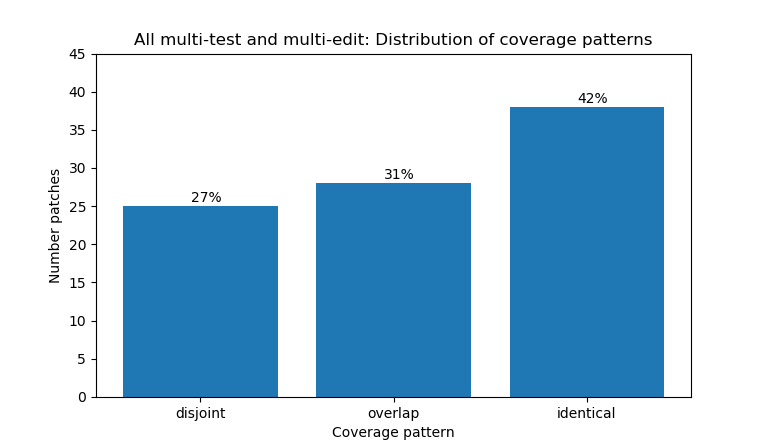
\includegraphics[width=\linewidth]{img/coverage-all.png}
	\caption{Distribution of coverage patterns for bugs with multiple failing
      tests that are repaired with multi-location patches in Bears and Defects4J.}
	\label{fig:coverage-all}
\end{figure}


\begin{figure}
	\begin{subfigure}{\linewidth}
		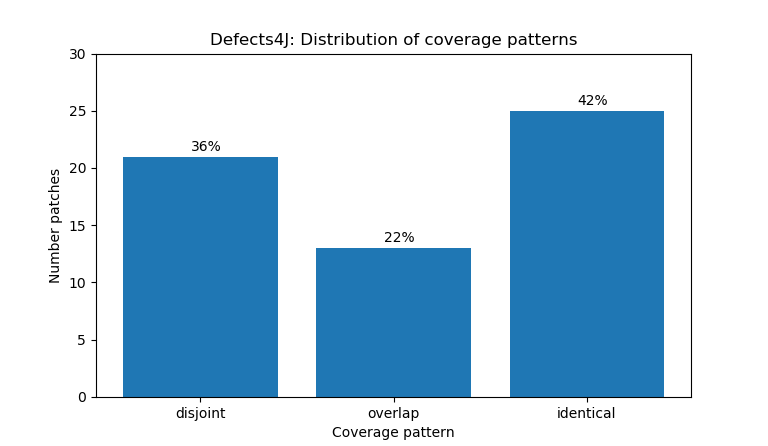
\includegraphics[width=\linewidth]{img/coverage-d4j.png}
		\caption{Distribution of coverage patterns for Defects4J.}
	\end{subfigure}

\vspace{0.5cm}

	\begin{subfigure}{\linewidth}
		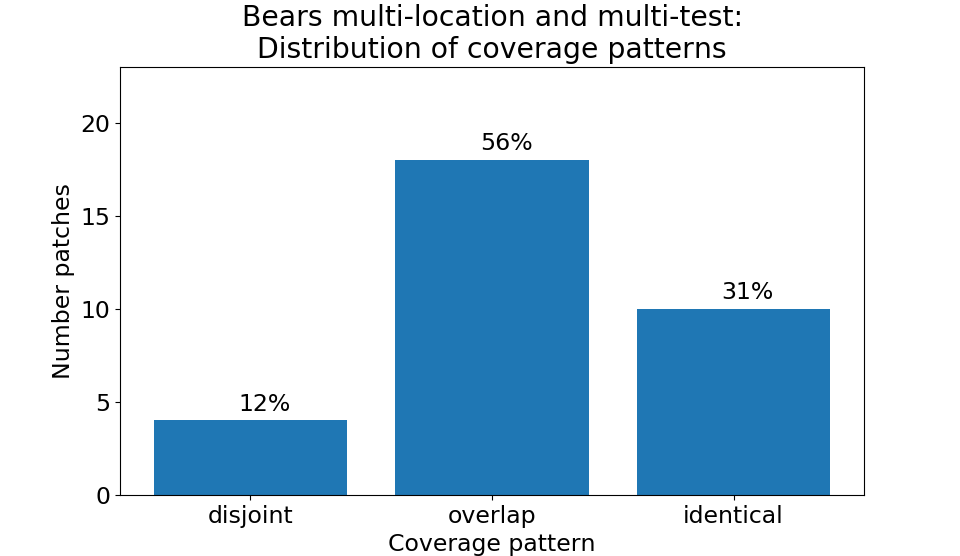
\includegraphics[width=\linewidth]{img/coverage-bears.png}
		\caption{Distribution of coverage patterns for Bears.}
	\end{subfigure}
	\caption{Distribution of coverage patterns by dataset,
          indicating significant differences between the multi-location bugs in
          Bears and Defects4J.}
	\label{fig:coverage-datasets}
\end{figure}

\subsection{Results}

\subsubsection{Distribution of Coverage Patterns} \label{sec:cov_patterns}

Figure~\ref{fig:coverage-all} shows results for the overall distribution,
combining the bugs in both datasets. 29\%
of the bugs were \emph{disjoint}.  Thus, for a significant portion of multi-location bugs,
none of the faulty lines were executed by all failing tests.  
In addition, another 39\% were classified as \emph{overlap}: only some of the
buggy locations were executed by all failing tests. In all, over half of 
the bugs that were both multi-location and multi-test contained edit locations that were 
not executed by all failing test cases.

Note, however, that the behavior varies considerably by dataset;
Figure~\ref{fig:coverage-datasets} shows results. In Defects4J, the patterns all have similar 
numbers of bugs, while in Bears, there are fewer \emph{disjoint} bugs and more 
\emph{overlap} 
bugs.
We hypothesize that this may be due to differences in how the two  
datasets were selected and constructed:
The Defects4J dataset specifically enforces a requirement that the patches in the 
dataset be isolated, i.e., not containing any refactorings or new features, to improve the 
usability of the dataset. The authors specifically chose patches that met this requirement, 
and in some cases, manually isolated the bug themselves~\cite{defects4j}. By contrast, the 
bugs in 
Bears are scraped directly from continuous integration systems, and the 
only requirements for inclusion is that the bug must be reproducible and that
the patch must be written by a human. In addition, Bears was designed to be evolvable 
and relatively easily expanded as a dataset, which is at odds with manual inspection and isolation of 
bugs~\cite{bears}.
Given that these two datasets were designed with different values and demonstrate very 
different behavior, these findings highlight the importance of using diverse datasets in 
evaluating program repair techniques.

Out of the 98 bugs we checked, only seven bugs had differing coverage patterns when 
classified based on coverage of patch lines vs. coverage of patch locations. All seven of these 
bugs 
were classified as \emph{overlap} when classified by line coverage, but were classified as 
\emph{identical} when classifying by patch coverage, indicating that all the failing tests were 
executing different paths within the same patch locations. \todo{Is this discussion confusingly 
worded? Because patch locations refer to the patch chunk, made up of one or more lines of 
code.}

Overall, SBFL assumes that faulty locations are executed more often by identifying 
or failing test cases and is not designed to find many of these multi-location
faults. Our results suggest that off-the-shelf SBFL techniques are not
well-suited to guiding APR techniques that conform to the dominant paradigm to repairing
these types of multi-location, multi-test bugs.

\begin{figure}
	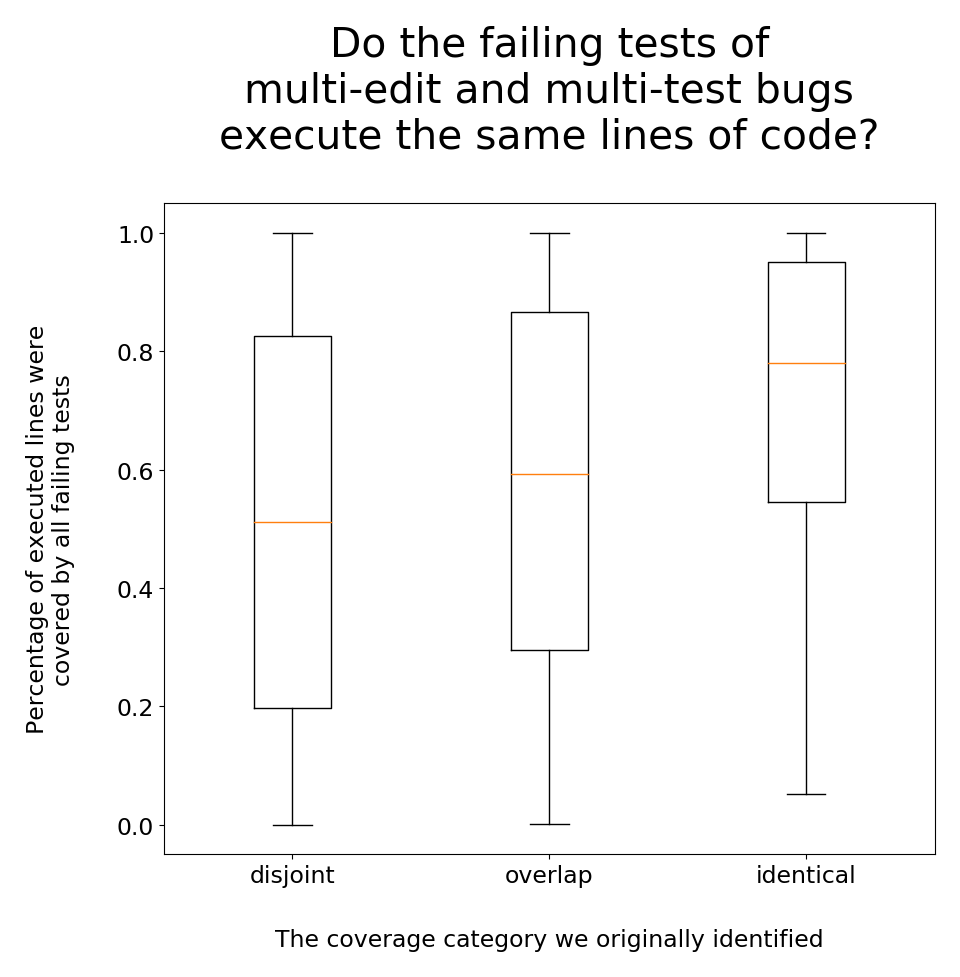
\includegraphics[width=.9\linewidth,left]{img/coverage-buggy.png}
	\caption{Boxplots representing the distribution of bugs based on it's percentage of lines 
	executed 
	by all failing tests. A bug scored at 100\% indicates that all failing tests executed the same 
	lines of 
	code, whereas a bug scored at 0\% indicates failing tests all executed different lines of 
	code. 
	These boxplots are split by coverage pattern, as categorized before.}
	\label{fig:coverage-buggy}
\end{figure}

\subsubsection{Identification of Coverage Patterns} \todo{There's a more accurate word 
here 
than "identification"}

Our results are shown in Figure \ref{fig:coverage-buggy}. Here, we see three distributions, 
separated by coverage pattern, and plotted based on the percentage of lines executed by all 
failing tests. We can see some qualitative differences between the three distributions. In 
particular, \emph{identical} bugs are more likely to have failing tests that execute the same lines 
of code, as we might expect. However, in practice, it would be difficult to determine the 
coverage pattern of a bug based on the coverage of failing tests alone, as all the distributions 
range from 5\% to 100\% (note that a bug categorized as disjoint can be scored 100\%, as the 
patch can introduce if statements that break the control flow and cause certain patch locations 
not to be executed). Thus, more work may be needed to identify the different coverage patterns 
from the buggy program.
